\documentclass{article}
\usepackage{tikz}

\begin{document}

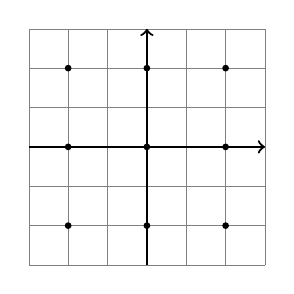
\begin{tikzpicture}[scale=0.5]
    % Draw the grid
    \draw[help lines] (0,0) grid (6,6);
    
    % Draw the axes
    \draw[->, thick] (3,0) -- (3,6);
    \draw[->, thick] (0,3) -- (6,3);
    
    % Mark the points
    \filldraw (1,1) circle (2pt);
    \filldraw (1,3) circle (2pt);
    \filldraw (1,5) circle (2pt);
    \filldraw (3,1) circle (2pt);
    \filldraw (3,3) circle (2pt);
    \filldraw (3,5) circle (2pt);
    \filldraw (5,1) circle (2pt);
    \filldraw (5,3) circle (2pt);
    \filldraw (5,5) circle (2pt);
\end{tikzpicture}

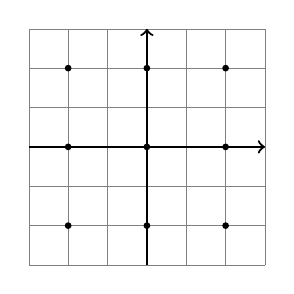
\begin{tikzpicture}[scale=0.5]
    % Draw the grid
    \draw[help lines] (0,0) grid (6,6);
    
    % Draw the axes
    \draw[->, thick] (3,0) -- (3,6);
    \draw[->, thick] (0,3) -- (6,3);
    
    % Mark the points
    \filldraw (1,1) circle (2pt);
    \filldraw (1,3) circle (2pt);
    \filldraw (1,5) circle (2pt);
    \filldraw (3,1) circle (2pt);
    \filldraw (3,3) circle (2pt);
    \filldraw (3,5) circle (2pt);
    \filldraw (5,1) circle (2pt);
    \filldraw (5,3) circle (2pt);
    \filldraw (5,5) circle (2pt);
\end{tikzpicture}

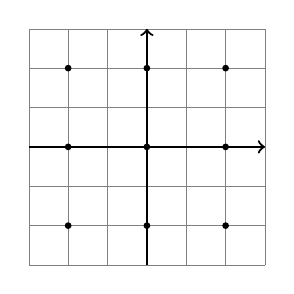
\begin{tikzpicture}[scale=0.5]
    % Draw the grid
    \draw[help lines] (0,0) grid (6,6);
    
    % Draw the axes
    \draw[->, thick] (3,0) -- (3,6);
    \draw[->, thick] (0,3) -- (6,3);
    
    % Mark the points
    \filldraw (1,1) circle (2pt);
    \filldraw (1,3) circle (2pt);
    \filldraw (1,5) circle (2pt);
    \filldraw (3,1) circle (2pt);
    \filldraw (3,3) circle (2pt);
    \filldraw (3,5) circle (2pt);
    \filldraw (5,1) circle (2pt);
    \filldraw (5,3) circle (2pt);
    \filldraw (5,5) circle (2pt);
\end{tikzpicture}

\end{document}